\let\negmedspace\undefined
\let\negthickspace\undefined
\documentclass[journal]{IEEEtran}
\usepackage[a5paper, margin=10mm, onecolumn]{geometry}

\usepackage{tfrupee} 
\setlength{\headheight}{1cm} 
\setlength{\headsep}{0mm}     

\usepackage{gvv-book}
\usepackage{gvv}
\usepackage{cite}
\usepackage{amsmath,amssymb,amsfonts,amsthm}
\usepackage{algorithmic}
\usepackage{graphicx}
\graphicspath{{figs/}}
\usepackage{textcomp}
\usepackage{xcolor}
\usepackage{txfonts}
\usepackage{listings}
\usepackage{enumitem}
\usepackage{mathtools}
\usepackage{gensymb}
\usepackage{comment}
\usepackage[breaklinks=true]{hyperref}
\usepackage{tkz-euclide} 
\usepackage{listings}

\def\inputGnumericTable{}                                 
\usepackage[latin1]{inputenc}                                
\usepackage{color}                                            
\usepackage{array}                                            
\usepackage{longtable}                                       
\usepackage{calc}                                             
\usepackage{multirow}                                         
\usepackage{hhline}                                           
\usepackage{ifthen}                                           
\usepackage{lscape}

\begin{document}

\bibliographystyle{IEEEtran}

\title{1.2.21}
\author{AI25btech11014- Suhas}

{\let\newpage\relax\maketitle}

\renewcommand{\thefigure}{\theenumi}
\renewcommand{\thetable}{\theenumi}
\setlength{\intextsep}{10pt}

\numberwithin{equation}{enumi}
\numberwithin{figure}{enumi}
\renewcommand{\thetable}{\theenumi}






\section*{Question}
\vspace{0.5cm}
The centroid of triangle $\triangle ABC$ is at the point $\vec{G} = \myvec{1\\1\\1}$.  
The coordinates of points $\vec{A}$ and $\vec{B}$ are given by:
\[
\vec{A} = \myvec{3\\-5\\7}, \quad \vec{B} = \myvec{-1\\7\\-6}
\]
Find the coordinates of point $\vec{C}$.

\section*{Solution}
\vspace{0.5cm}
The centroid $\vec{G}$ of triangle $\triangle ABC$ is given by the formula:
\[
\vec{G} = \frac{1}{3}(\vec{A} + \vec{B} + \vec{C})
\]

Multiplying both sides by 3:
\[
3\vec{G} = \vec{A} + \vec{B} + \vec{C}
\]

Solving for $\vec{C}$:
\[
\vec{C} = 3\vec{G} - \vec{A} - \vec{B}
\]

\subsection*{Symbolic Expression}

Let $\vec{A} = \vec{a}$, $\vec{B} = \vec{b}$, and $\vec{G} = \vec{g}$, then:
\[
\vec{C} = 3\vec{g} - \vec{a} - \vec{b}
\]

\subsection*{Numerical Substitution}

Substitute the given values:
\[
\vec{C} = 3\myvec{1\\1\\1} - \myvec{3\\-5\\7} - \myvec{-1\\7\\-6}
\]

Compute step-by-step:
\[
3\vec{G} = \myvec{3\\3\\3}
\]
\[
\vec{C} = \myvec{3\\3\\3} - \myvec{3\\-5\\7} = \myvec{0\\8\\-4}
\]
\[
\vec{C} = \myvec{0\\8\\-4} - \myvec{-1\\7\\-6} = \myvec{1\\1\\2}
\]

\subsection*{Final Answer}

The coordinates of point $\vec{C}$ are:
\[
\vec{C} = \myvec{1\\1\\2}
\]


















\newpage
\begin{figure}[h!]
   \centering
   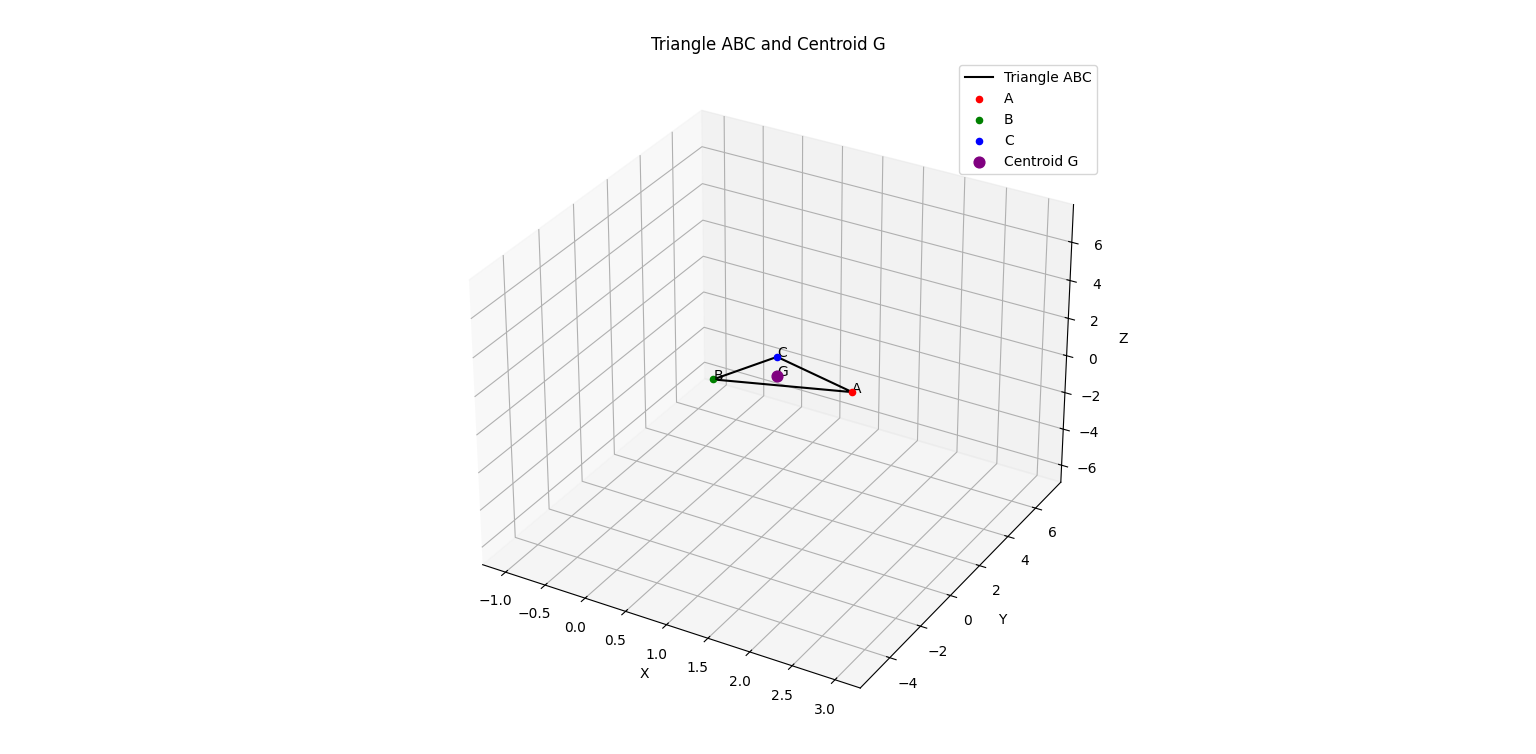
\includegraphics[width=1\linewidth]{figs/fig1.png}
   \caption{3D plot of triangle ABC and centroid G}
   \label{}
\end{figure}

\end{document}